\documentclass[border=4pt]{standalone}
\usepackage[dvipsnames,svgnames]{xcolor}
\usepackage{tkz-tab}
\definecolor{fondpaille}{cmyk}{0,0,0.1,0}
\begin{document}
% test exhaustif des clés
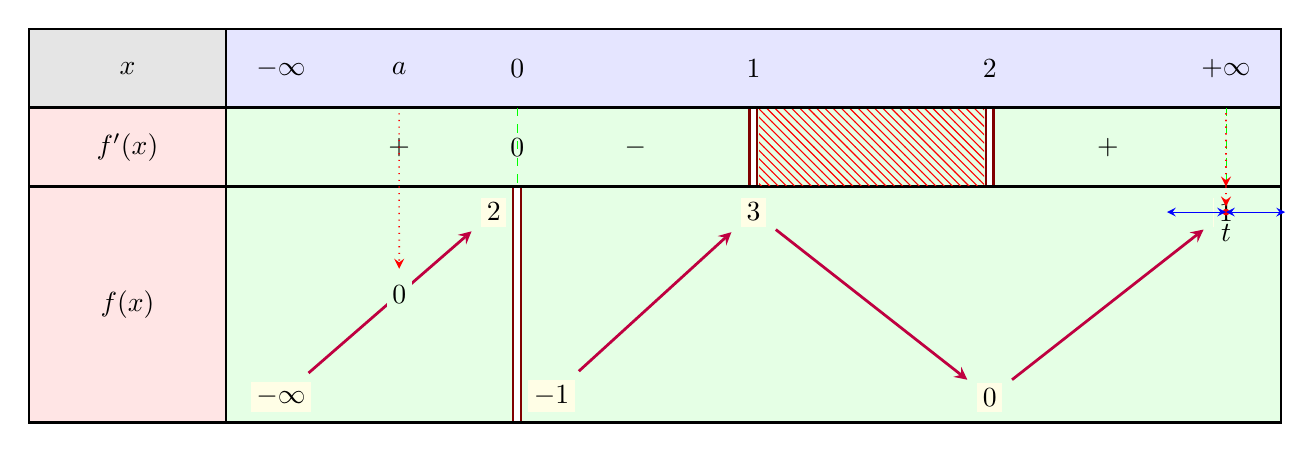
\begin{tikzpicture}
\tkzTabColors[color=blue,backgroundcolor=yellow!10]
\tkzTabSetup[crosslines,doubledistance=2pt,lw=0.8pt,doublecolor=white,color=Maroon,
  backgroundcolor=fondpaille,patterncolor=red,patternstyle=north east lines,
  tstyle=dashed,tcolor=green,tanstyle=<->,tanarrowstyle=stealth,tancolor=blue,
  tanwidth=1pt,fromstyle=->,fromarrowstyle=stealth,fromcolor=red,fromwidth=0.6pt,
  twidth=0.3pt,hcolor=orange,hopacity=0.6,arrowcolor=purple,arrowstyle=stealth,
  arrowlinewidth=1pt,,]
\tkzTabInit[color,lw=1pt,colorC=red!10,colorL=blue!10,colorT=green!10,colorV=gray!20,
   lgt=2.5,textw=2,espcl=3,deltacl=0.7]
  {$x$/1,$f'(x)$/1,$f(x)$/3}{$-\infty$,$0$,$1$,$2$,$+\infty$}
\tkzTabLine{,+,z,-,d,h,d,+,t}
\tkzTabVar[color=red]{-/$-\infty$,+D-/$2$/$-1$,+/$3$,-/$0$,+/$1$}
\tkzTabVal[draw,remember=v1]{1}{2}{0.5}{$a$}{$0$}
\tkzTabIma[draw,remember=v2]{4}{5}{5}{$1$}
\tkzTabTan[draw,color=red,pos=below,remember=v3]{4}{5}{5}{$t$}
\end{tikzpicture}
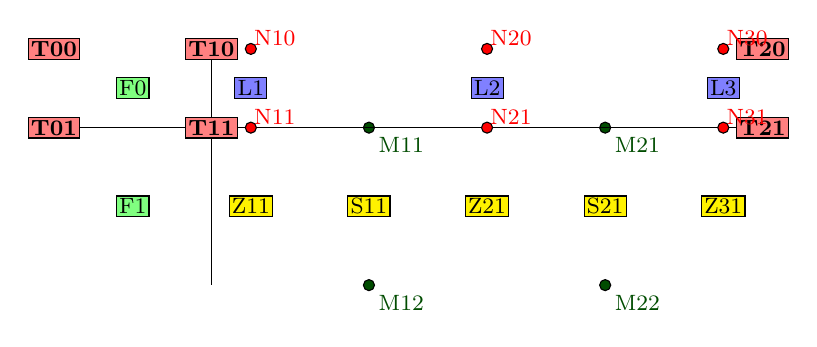
\begin{tikzpicture}[yshift=-8cm]
\tkzTabSetup[doubledistance=3pt]   % doit remettre toutes les autres clés à leur défaut
\tkzTabInit[nocadre,help]{$x$/1,$g$/2}{$0$,$1$,$2$}
\tkzTabLine[help]{,+,z,-,}
\end{tikzpicture}
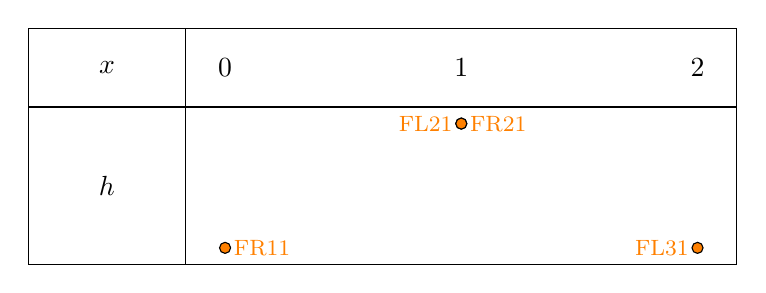
\begin{tikzpicture}[yshift=-14cm]
\tkzTabInit{$x$/1,$h$/2}{$0$,$1$,$2$}   % pas d'options : défauts
\tkzTabVar[help]{-/$0$,+/$1$,-/$0$}
\end{tikzpicture}
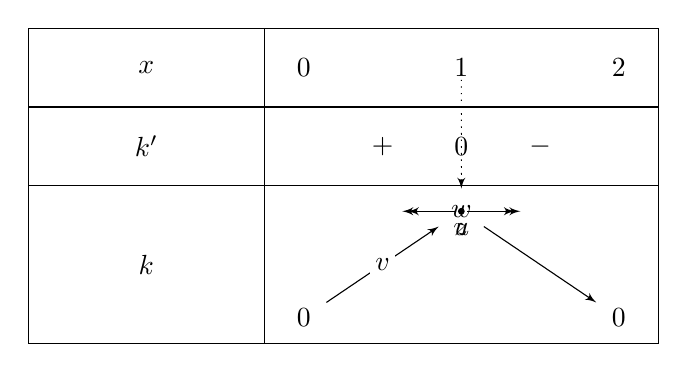
\begin{tikzpicture}[yshift=-20cm]
\tkzTab[lgt=3,espcl=2]{$x$/1,$k'$/1,$k$/2}{$0$,$1$,$2$}{,+,z,-,}{-/$0$,+/$1$,-/$0$}
\tkzTabTan[pos]{1}{2}{2}{$u$}
\tkzTabVal{1}{2}{0.5}{}{$v$}
\coordinate (Q) at (L2);
\tkzTabImaFrom[draw]{2}{3}{Q}{$w$}
\tkzTabTanFrom[pos=below]{2}{3}{Q}{$z$}
\end{tikzpicture}
\end{document}
